% DNS defined in the intro!
\subsection{Incompressible DNS Application}
\label{sec:dns_full}

% Why DNS code needs to be improved
Direct numerical simulation (DNS) plays an important role in understanding turbulent flows because DNS provides high fidelity data that is difficult to obtain in the experiments. After Kim {\it et al.} first used the DNS for wall-bounded turbulence flow in 1987 \cite{Kim:1987ub}, DNS has been used extensively to understand the turbulence phenomenon and to help develop models of turbulence. In general, the length-scale and time-scale become smaller as $Re$ increases where $Re$ is Reynolds number. Naturally, DNS at high $Re$ requires a large number of grids and time-steps to obtain meaningful statistical data. Therefore, the use of state-of-art HPC system is crucial to study the turbulent flow of high Re. To date, the highest $Re$ of the wall-bounded turbulence DNS is 250000, for which 242 billion degrees of freedom are used. \cite{Lee:2015er} However, $Re$ = 250000 is also low compared to the high Re flow required for many practical engineering applications. For a DNS at higher Re, more advanced HPC system is required, and the DNS code should also be improved for the the HPC system.

% Detail of simulation
In this section, we will show you the results of testing PoongBack on KNL nodes in Stampede, which is a channel flow DNS code optimized for the modern HPC systems. PoongBack simulates the flow between two parallel plates with periodic boundary conditions. The simulation code has already shown excellent performance and has been already used in several researchers. \cite{Lee:2013kv} Especially, it has been used for generating the data for virtual flow laboratory in Johns Hopkins Turbulence Data Base \cite{Graham:2015ha}.It is using Fourier-Galerkin method in streamwise direction and high order basis spline method in wall-normal directions. For time integration PoongBack uses low-storage third order Runge-Kutta method. The simulation domain is partitioned by two-dimensional decomposition, a.k.a. pencil-decomposition. PoongBack contains three major kernels; (1) solving Navier-Stokes equation in complex number domain (2) one-dimensional fast Fourier transforms (3) data transpose in two dimension. The combination of (2) and (3) makes 3D FFT and there are multiple libraries for it. We developed customized 3D FFT library because of the needs of zero-padding for 3/2 dealiasing. Additionally, PoongBack uses customized I/O library for HDF5 format, ESIO \cite{Lee:2014ta}, but the I/O performance is not the scope of current work. See \cite{Lee:2013kv,Lee:2014ta} for more detail about PoongBack.  

For this study the grid size is used $1024\times128\times512$ and the grid size is comparable for $Re_\tau = 180$ simulation by \cite{Kim:1987ub}. Throughout the every benchmark cases, the MCDRAM is used as a cache memory between processors and DRAM. The simulation code is compiled with a flag ``{\tt -xMIC-AVX512}.'' Also, the FFTW-3.3.5 library is installed with the options ``{\tt --enable-avx512}'' and ``{\tt --enable-mpi}.'' \cite{Frigo:2005tu} We used double-precision operation for all kernels and elapsed times were measured by ``{\tt mpi\_wtime()}'' with appropriate ``{\tt mpi\_barrier()}.''

\begin{figure}[htb]
 \begin{center}
   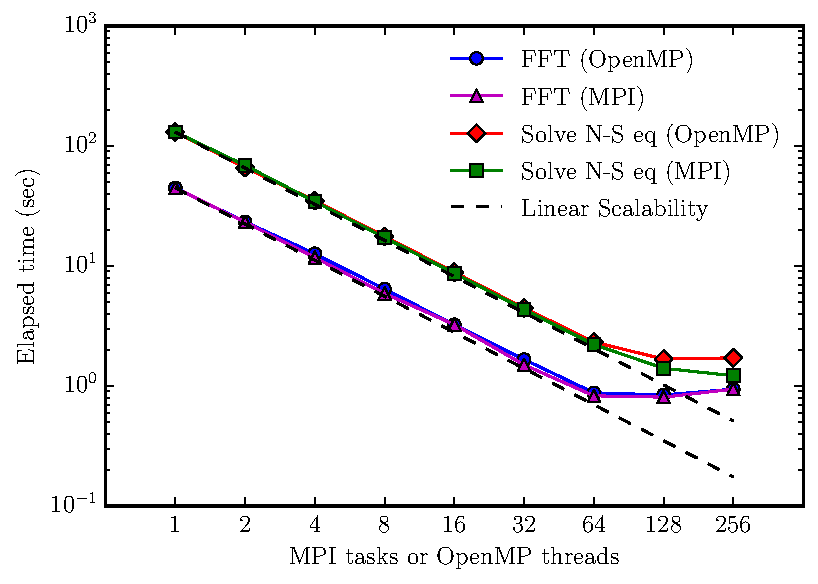
\includegraphics[width=0.45\textwidth]{DNS_FFT_Wave}
   \caption{Strong scaling result of 1D FFTs and Solving N-S equations in wavespace for single timestep.}
   \label{fig:DNS_strong_scale_fft_wave}
 \end{center}
\end{figure}

% 1D FFT and wavespace performance
Figure~\ref{fig:DNS_strong_scale_fft_wave} shows the strong scaling performance of the kernels involving floating point operations; 1D FFTs and solving Navier-Stokes equation. Four different FFTs are performed; real-to-complex (R2C), complex-to-real (C2R), forward complex-to-complex (fC2C) and backward complex-to-complex (bC2C). Before or after each FFTs zeroes in the half length of 1d contiguous data lines are padded or truncated. Also, nonlinear products such as $A\times B \rightarrow C$ are performed between C2R and R2C transforms. The elapsed time for 1d FFTs, zero padding/truncation and nonlinear product is shown in figure~\ref{fig:DNS_strong_scale_fft_wave} as FFT. In both case of using MPI only and OpenMP only the performance is almost linear up to 64 processors are used. When two hardware threads were used per core, the performance did not increased. Also, the performance decreases when four hardware threads were used in both MPI and OpenMP cases. The performance was the best with 64 processors and showed 270 GFlops which is approximately 9\% of peak performance. It means that the performance of 1D FFTs on KNL nodes are memory bandwidth bounded. There are numerous floating point operation involved in the kernel of solving Navier-Stokes equation. Solving linear equations $A \textbf{x} = \textbf{b}$ and matrix-vector multiplications are the most important parts in the kernel. Here, the matrix $A$ is in a form of banded matrix with additional non-zero elements in several first and last rows. Also, the elements of $A$ are real whereas the elements of $\textbf{x}$ and $\textbf{b}$ are complex. Because of these properties, we have implemented customized linear algebra solver. Since the Navier-Stokes equation is solved in complex number domain after 1d FFTs in two directions, 3D PDE becomes 1D ODE at each wavenumbers. Hence, the Navier-Stokes equation can be solved at each wavenumbers without interaction with the data in other wavenumbers. As a result, the kernel can be parallelized and requires no communication. The performance of the kernel of solving Navier-Stokes equation is shown in figure~\ref{fig:DNS_strong_scale_fft_wave} as Solve N-S eq. Similar to FFT, both MPI only and OpenMP only cases shows almost ideal scalability up to 64 cores. There were small, but noticeable, performance increases observed with two hardware threads. Interestingly, the performance of OpenMP only case decreases while the performance of MPI only case increases when four hardware threads per core were applied. This maybe due to the difference of memory access pattern between two parallelism or scheduling overhead in OpenMP. \todo{MK:Please tell me if this explanation is reasonable.}         

% Transpose performance
\begin{figure}[htb]
 \begin{center}
   \includegraphics[width=0.45\textwidth]{DNS_Transpose}
   \caption{Strong scaling result of data reorder and MPI communication; OpenMP is not used.}
   \label{fig:DNS_strong_scale_transpose}
 \end{center}
\end{figure}

The last kernel of PoongBack is the data transpose in two dimensionally partitioned domain. This kernel is for the data alignment for FFTs and linear problems in solving Navier-Stokes equation and does not include any floating point operations. However, more than 50\% of simulation time is spent for this operation. The data transpose kernel includes two subsequent parts; (1) All-to-All type MPI communication in two sub-communicators. (2) The data reordering to maximize message size of MPI and to finalized memory alignment after MPI communication. Since the domain is partitioned in two dimension, MPI communication needs to be performed in two dimension with MPI-sub-communicators. The communication in each direction is logically All-to-All, but other communication patterns can be faster than ``{\tt mpi\_alltoall}'' because 2D communication topology. We have used MPI-enabled FFTW (ver 3.3 or higher) to find the optimal communication patterns for each sub-communicator. Since MPI-enabled FFTW only support one dimensionally partitioned domain, a.k.a plane decomposition, we have separately used FFTW for 1D FFTs and MPI communications with ``{\tt fftw\_mpi\_execute\_r2r()}''. (This idea is originally from Dr. Rhys Ulerich.) The part of code for data reordering basically performs tensor transpose, such as {\tt B(i,j,k,l) $\leftarrow$ A(l,i,k,j)} or {\tt B(i,j,k) $\leftarrow$ A(j,k,i)}. Unfortunately, the cache-line optimization cannot be achieved for both load and store at the same time. In this work we chose the order of transpose prefer to load of cache lines. The performance of MPI communication and data reordering is shown in figure~\ref{fig:DNS_strong_scale_transpose}. Similar to FFTs and solving Navier-stokes equation, data reordering also shows almost linear scalability up to 64 cores. Also, the performance keep increases even with hardware threading. On the other hand, MPI communication shows performance increases as number of cores increases even with additional MPI tasks on the hardware threads, but the scalability is distant from linear. This is somewhat interesting because the code benchmark result on other HPC systems shows that MPI communication takes more than five times of the elapsed time for data reordering. \cite{Lee:2013kv} This may imply that the performance could be increased by fine tuning of data reordering for KNL nodes.

\begin{figure}[htb]
 \begin{center}
   \includegraphics[width=0.45\textwidth]{DNS_Parallelism}
   \caption{Comparison of MPI$\times$OpenMP in data transpose}
   \label{fig:DNS_MPI_OpenMP}
 \end{center}
\end{figure}


In data transpose kernel, OpenMP can be implemented in data reordering but not in MPI communication. The hybrid parallelism with MPI + OpenMP is tested and results are shown in figure~\ref{fig:DNS_MPI_OpenMP}. Each line in figure~\ref{fig:DNS_MPI_OpenMP} the cases where the product of the number of MPI tasks and the number of OpenMP threads is constants. Using more MPI tasks and less OpenMP threads generally shows better performances. The best performance is achieved when 256 MPI tasks were used at four hardware threads. This is because using MPI shows better performance than OpenMP for data reordering. Also, using more MPI tasks performs better for MPI communication as shown in figure~\ref{fig:DNS_strong_scale_transpose}. Finally, the size of tensor transpose changes with number of MPI tasks. 


\begin{figure}[htb]
 \begin{center}
   \includegraphics[width=0.45\textwidth]{DNS_full_timestep}
   \caption{Strong scaling result of total elapsed time for single timestep; (MPI tasks $\times$ OpenMP threads) is hybrid parallelism which shows the best performance.}
   \label{fig:DNS_strong_scale_total_elapsed_time}
 \end{center}
\end{figure}

The performance of one full timestep (without I/O) is shown in figure~\ref{fig:DNS_strong_scale_total_elapsed_time}. The best performance with different MPI $\times$ OpenMP with each number of processors is chosen.  It also shows almost perfect scalability up to 64 processors. The performance keeps increasing after using hardware threads. In most cases, using only MPI tasks shows the best performance excepts for 64 processors with 2 hardware threads. However the difference between hybrid parallelism and only MPI tasks are minimal for 128 processors. As a conclusion, using only MPI seems to be the best option for given problem size. We would like to note that hybrid parallelism should be still remained as an option. When the problem size is bigger than the size of DRAM of KNL node, one must use multiple KNL nodes. Using many MPI tasks can easily saturate the capability of interconnect device. In such condition, reducing the number of MPI tasks by using OpenMP could show better performance.  

\todo{if we merge this with the previous section, we can have an intro
to dns and then talk about each in detail}

